\clearpage
\section{UML Class Diagrams}

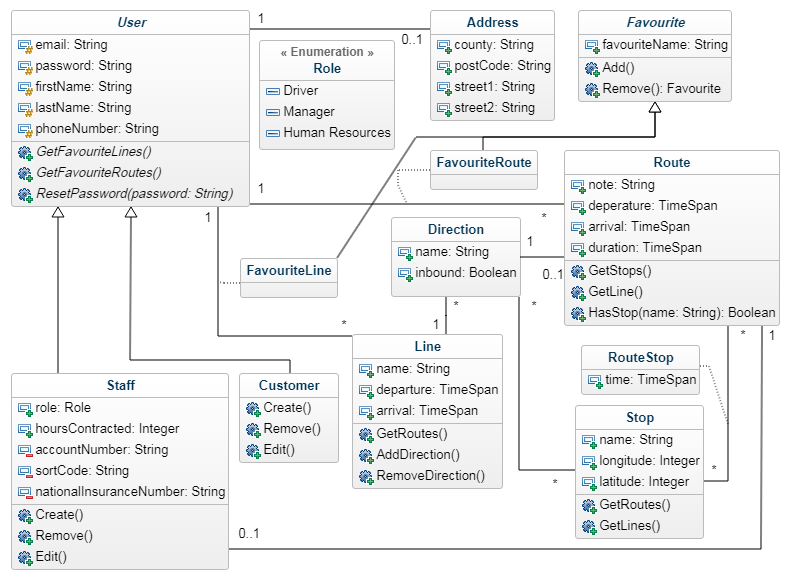
\includegraphics[width=\linewidth]{UMLClassDiagram.png}

\medskip

Functionally equivalent to the $ER$ diagram, the $User$ class is an
abstract class, which the $Staff$ class is generalised from.

\medskip

As $FavouriteLine$ and $FavouriteRoute$ share the same attributes
and methods, these classes are also a generalisation of an abstract
$Favourite$ class. As these two and $RouteStop$ are just associating
data from two tables, these are displayed as association classes in
the UML class diagram instead of regular classes.

\medskip

The $Staff$ class has $GetXHours()$ methods which calculate the hours
the staff member will be working within the duration ($day$, $week$ or
$month$) from the $hoursContracted$ for non-driver staff or route
durations the driver is assigned to. This will be used as validation
when assigning a driver to new routes, as a driver legally cannot
drive for more than 9 hours a day, plus the required breaks (with 2
days a week where they can drive 10 hours). If the route will cause
the driver to exceed the limit, the creation/edit view should
display an unobtrusive error and prevent confirming the change or
addition.

\medskip

The $Route$ class has a $GetStops()$ method which will be used by
the $Route Details$ and $Route Editing$ views to list all stops
associated with the selected route. $HasStop()$ will be used by the
homepage search, so only routes that service both selected stops
will be shown in the results.
